\documentclass[]{article}

\usepackage{enumitem}
\usepackage{ulem}

\usepackage{graphicx}
\graphicspath{ {./images/} }

\usepackage{tikz}
\usepackage{circuitikz}
\usepackage{tikz-qtree}
\tikzset{every tree node/.style={align=center}}

\usepackage{listings}

\usepackage{xcolor}
\definecolor{codegreen}{HTML}{859900}
\definecolor{codegray}{HTML}{839496}
\definecolor{codepurple}{HTML}{6C71C4}
\definecolor{codemagenta}{HTML}{d33682}
\definecolor{backcolour}{HTML}{FDF6E3}
\definecolor{fontcolor}{HTML}{002B36}
\lstdefinestyle{mystyle}{
	basicstyle=\color{fontcolor},
	backgroundcolor=\color{backcolour},   
	commentstyle=\color{codegreen},
	keywordstyle=\color{codemagenta},
	numberstyle=\tiny\color{codegray},
	stringstyle=\color{codepurple},
	breakatwhitespace=false,         
	breaklines=true,                 
	captionpos=b,                    
	keepspaces=true,                 
	numbers=left,                    
	numbersep=5pt,                  
	showspaces=false,                
	showstringspaces=false,
	showtabs=false,                  
	tabsize=8
}

\lstset{style=mystyle}

\title{Lab 2\\Arduino Basics}
\author{Keaton Clark}

\begin{document}
\maketitle

\section{Circuit}
\begin{center}
\begin{circuitikz}
	\draw (0,0) to 
		[short,l={$D_2$},o-](2,0) to 
		[push button](2,-2) to 
		[short,-o,l=5v](0,-2)
	;
	\draw (2,0) to
		[R=$1k\Omega$](2,2) to
		(0,2)node[ground]{}
	;
	\draw (6,0) to
		[short,l={$D_4$},o-](6,2) to
		[empty diode](4,2) to
		[R=$330\Omega$](2,2)
	;
\end{circuitikz}
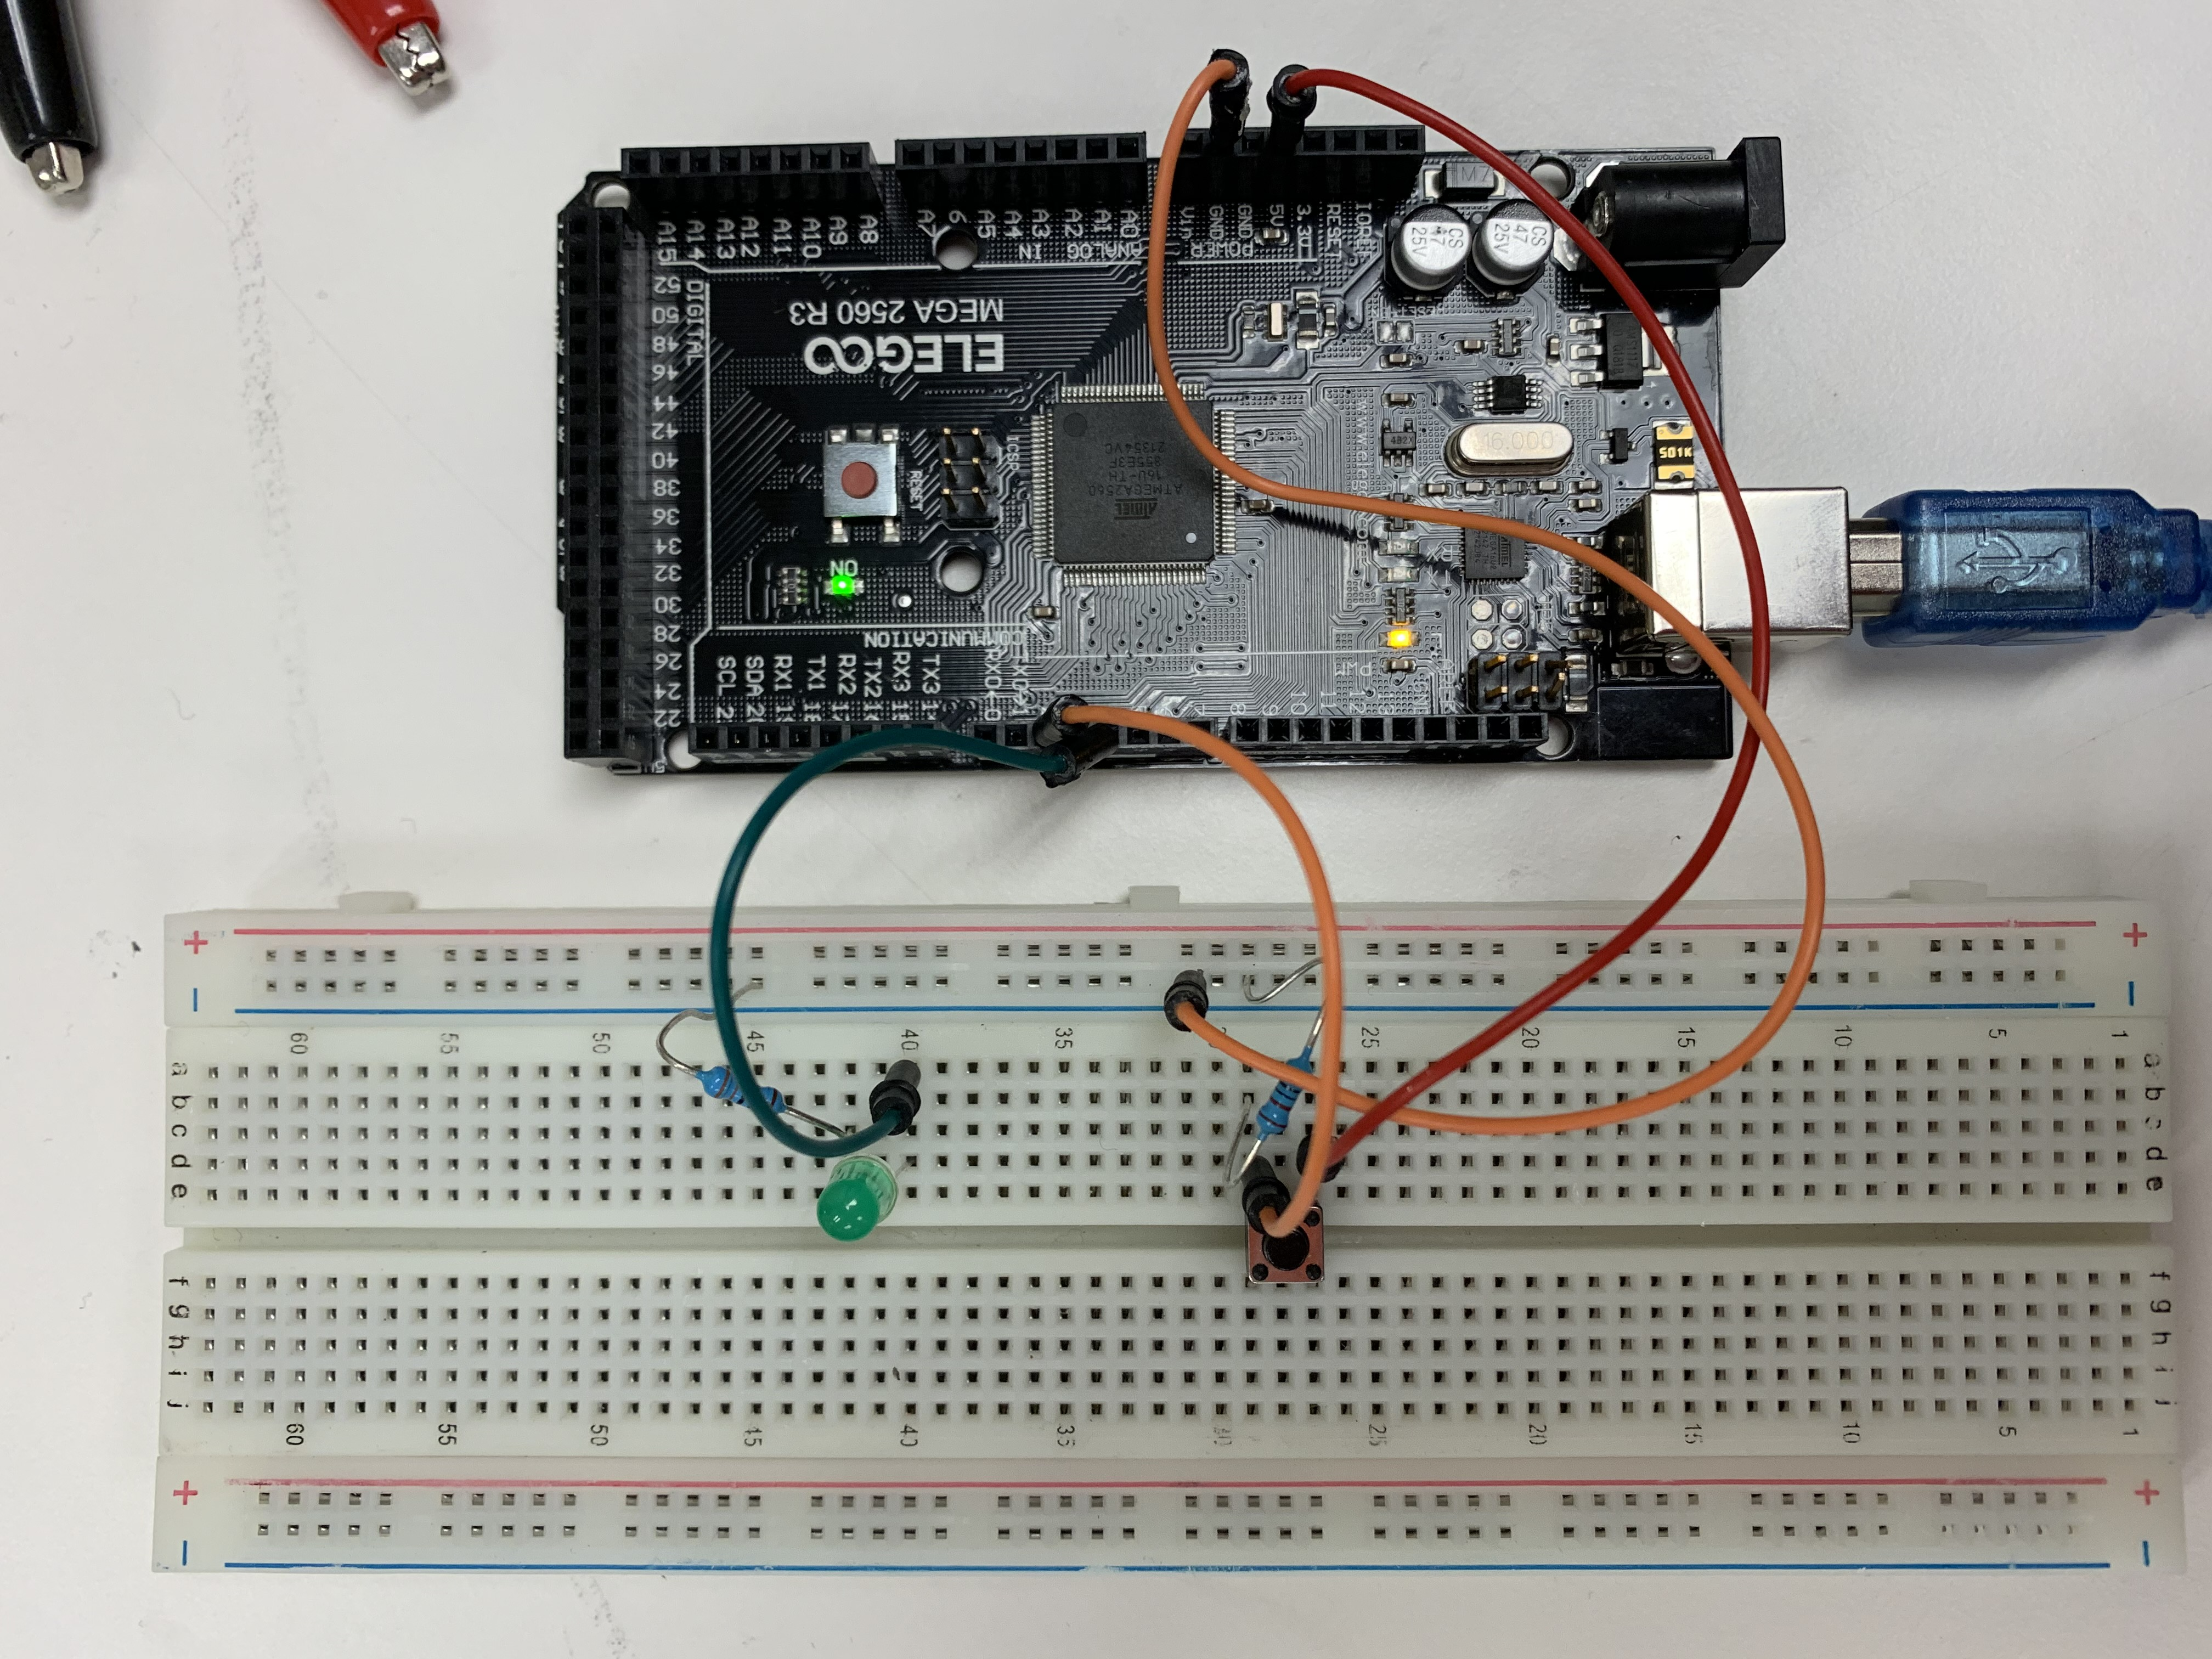
\includegraphics[scale=.05]{1.jpg}
\end{center}
\pagebreak
\section{Code}
main.c
\lstinputlisting[language=C]{../src/main.c}
The remainder of the source code is included under ./src

\pagebreak
\section{Results}
\begin{center}
	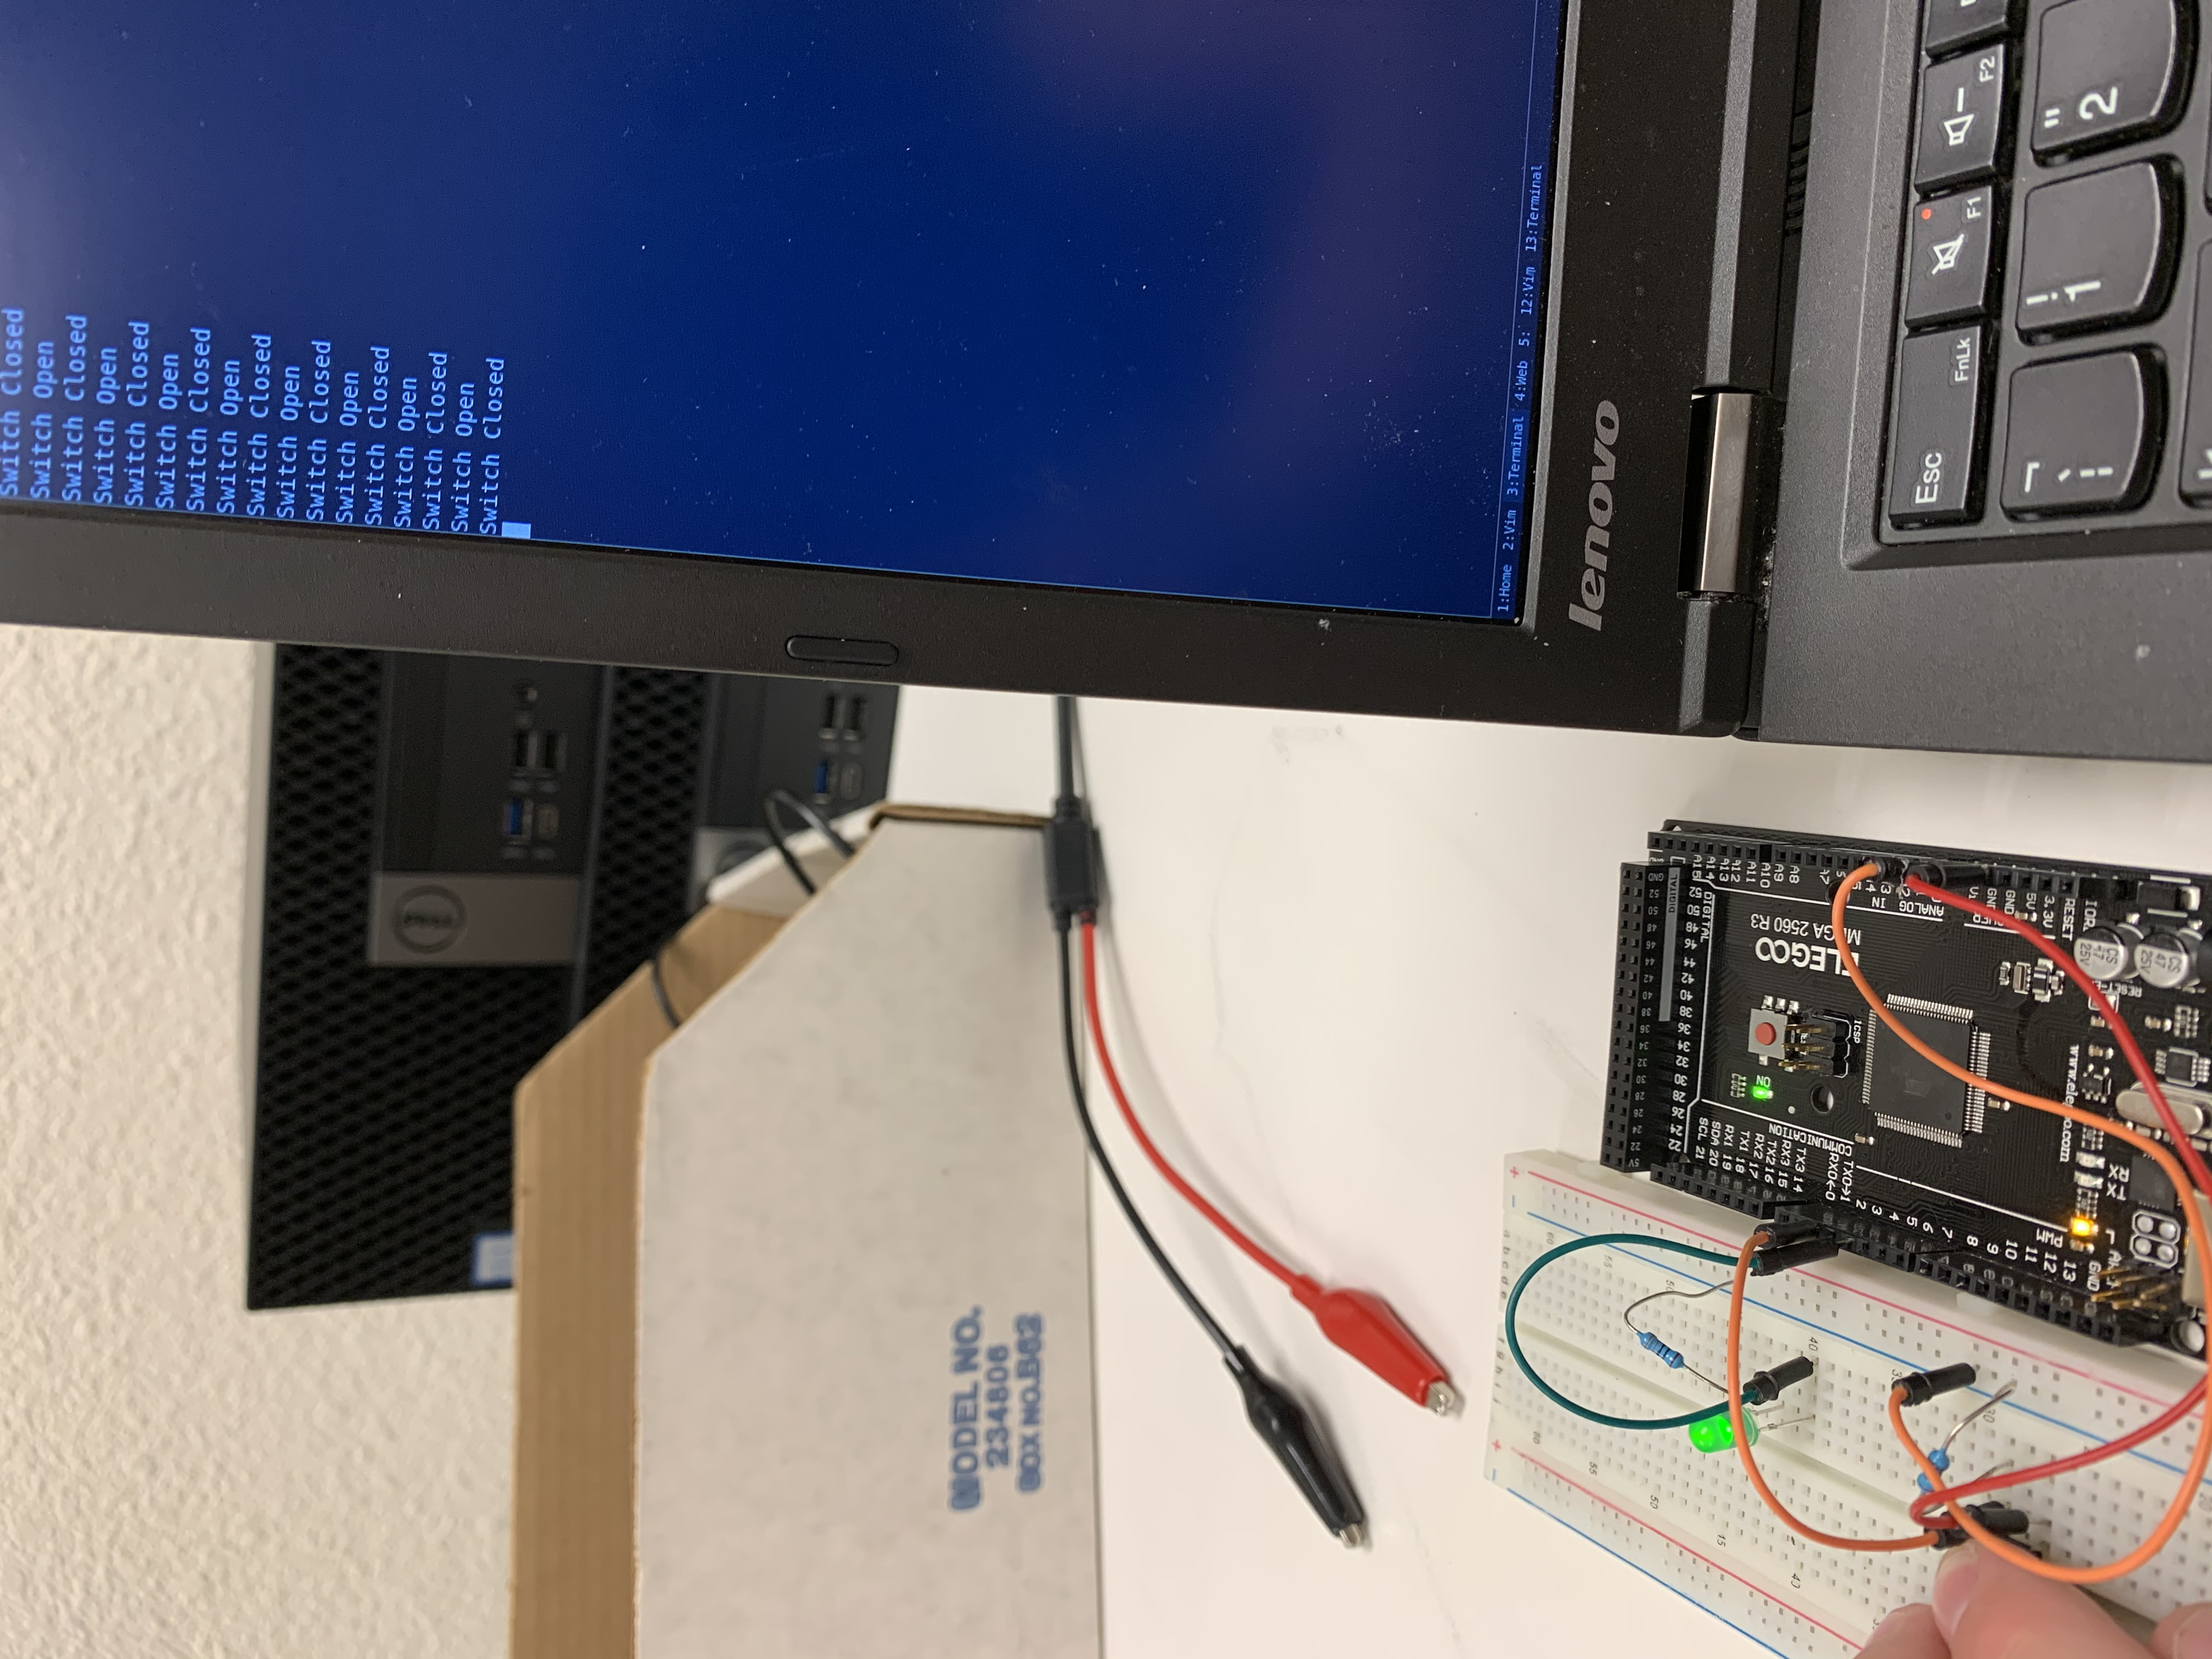
\includegraphics[scale=.06,angle=-90]{2.jpg}\\
	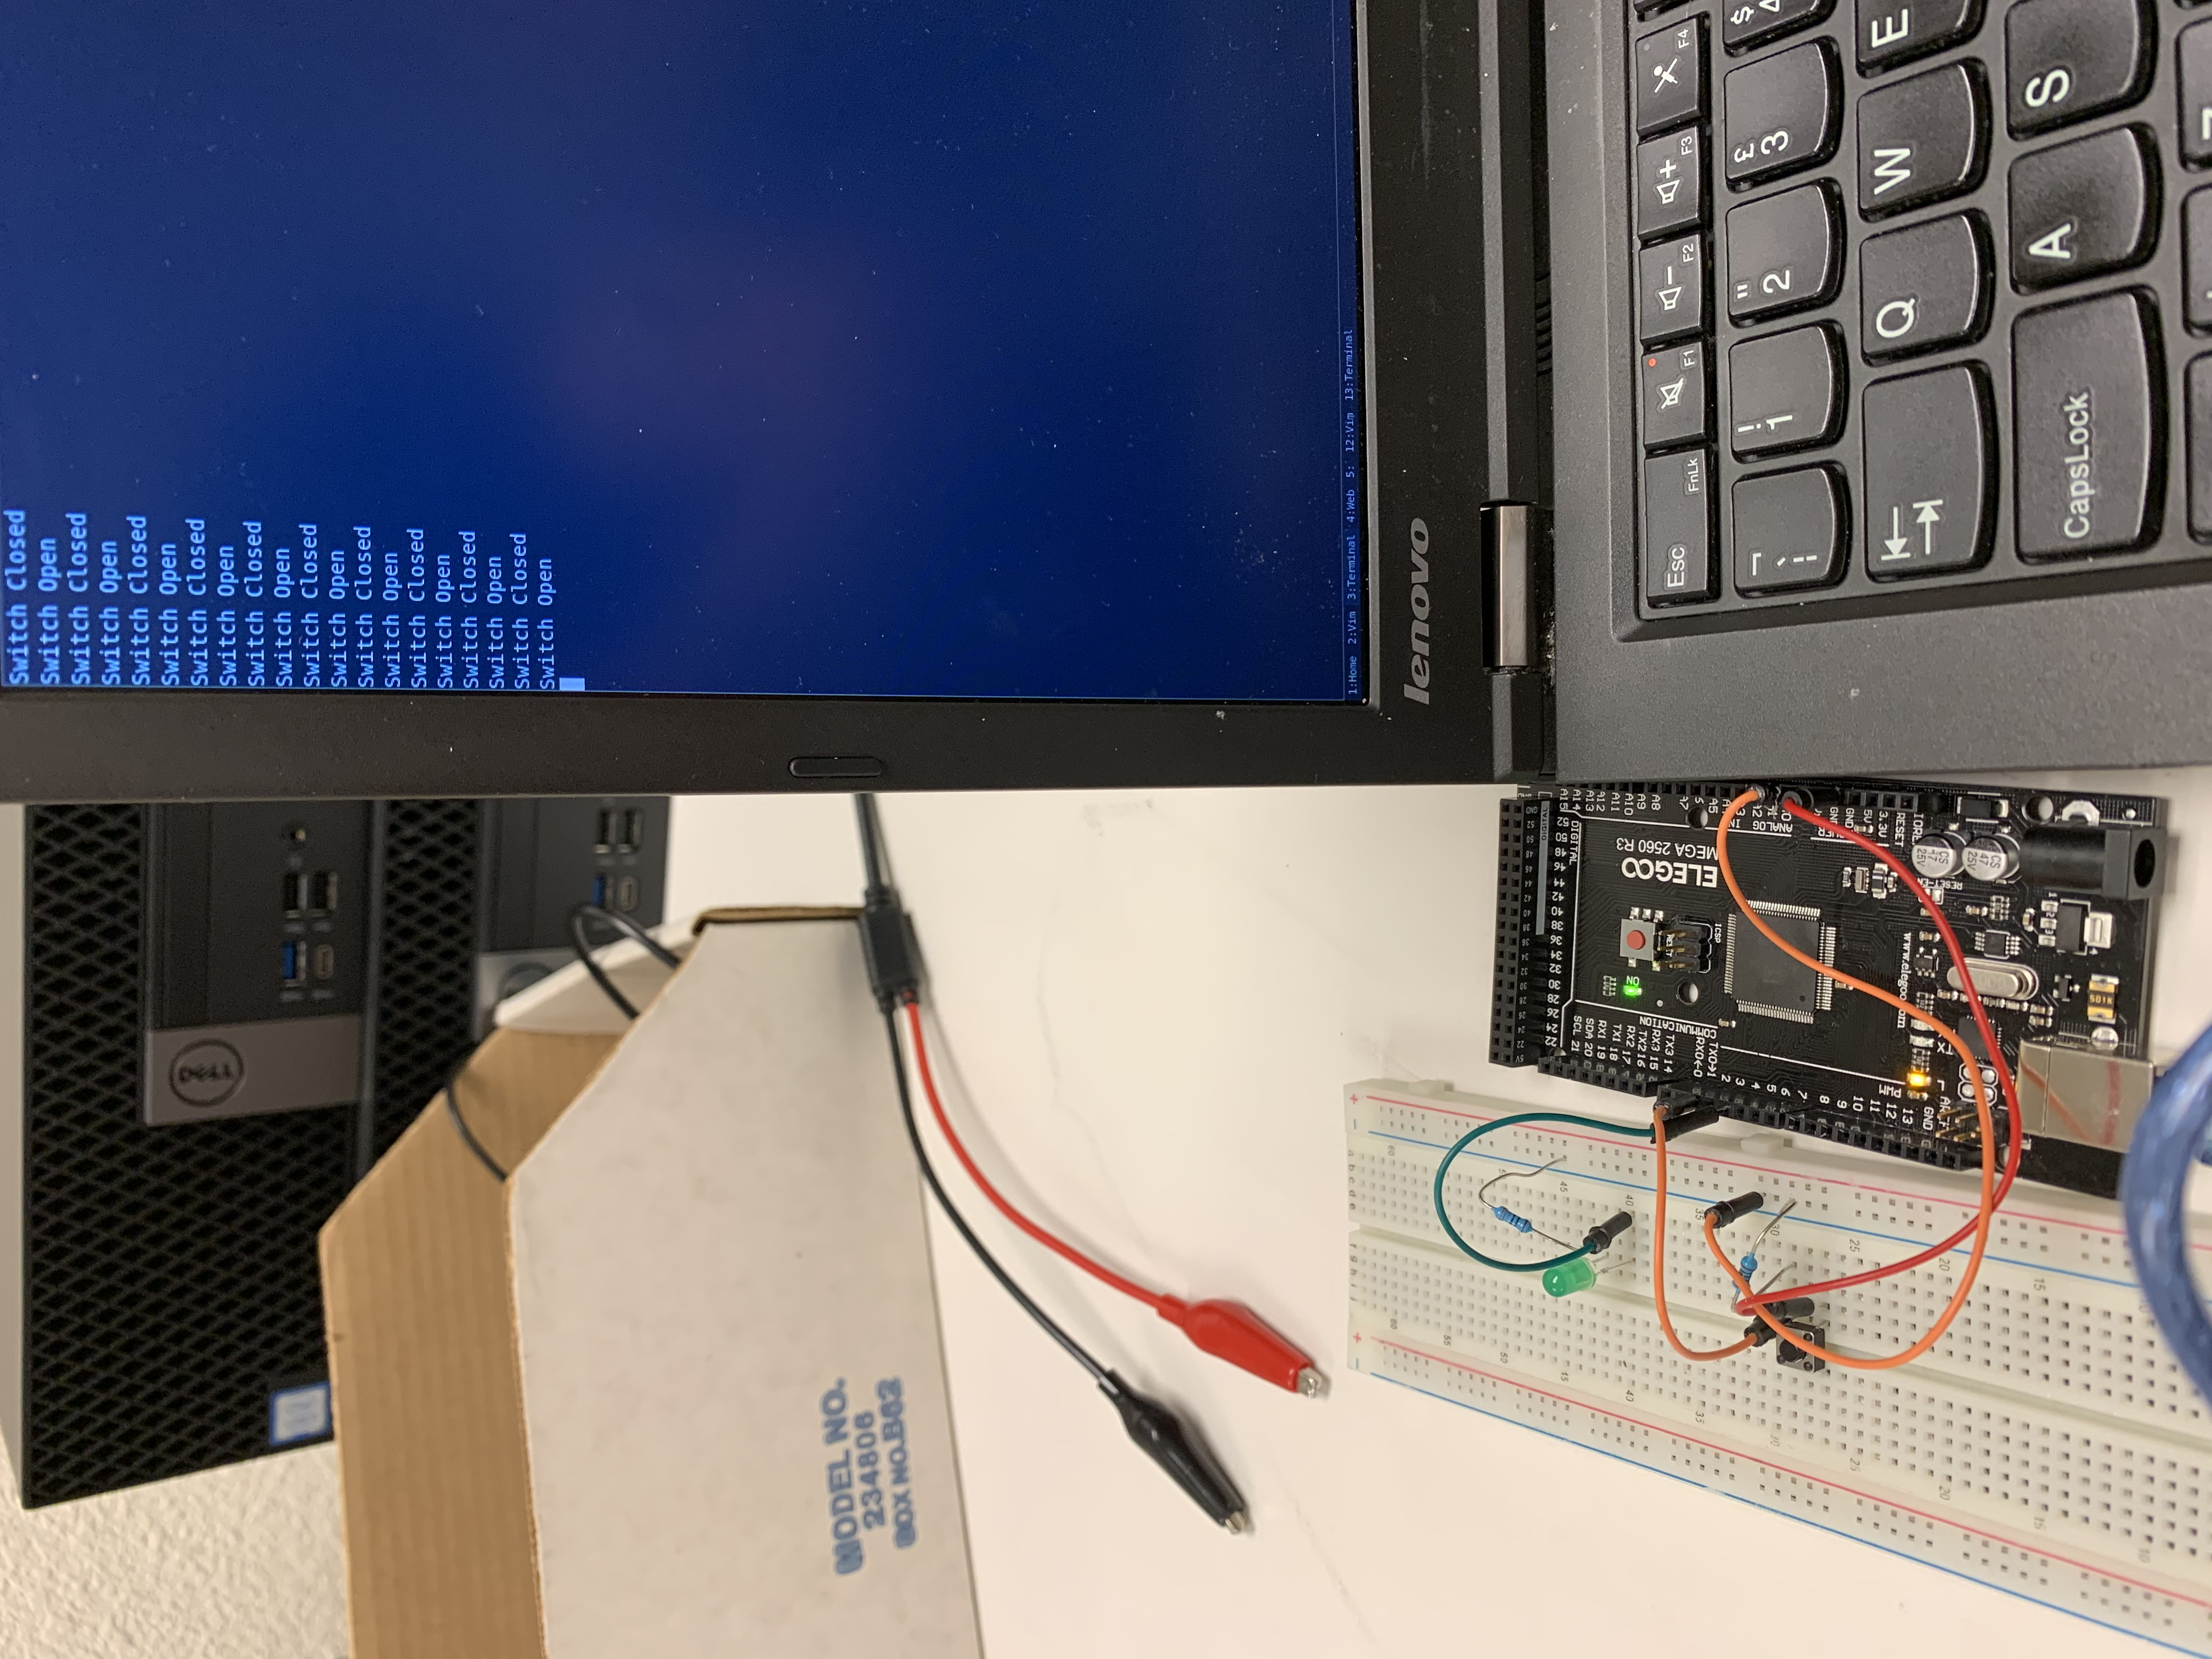
\includegraphics[scale=.06,angle=-90]{3.jpg}
\end{center}
\pagebreak
\section{Questions}
\begin{enumerate}
	\item A pin on the Arduino is a semi-arbitrary number assigned to a pin on the microcontroller present on the specific model of Arduino.
	This helps us to more easily interface with the microcontroller through the Arduino IDE.
	\item The serial port is in reference to the UART communication you are able to use on the ATMEGA2560 which is a type of serial communication that works with two lines to transmit and receive at the same time.
	On the Arduino Mega 2560 this is actually communicating with a second microcontroller (ATMEGA16u2) which then handles communication through USB.
	\item Analog data is transmitted by a variable voltage, on the Arduino it is 0-5v, and can be expressed as a range of values correlating to the ratio of the signal voltage to the maximum readable voltages.
	Digital on the other hand is simply the presence or absence of a signal with 0v correlating to a 0 and any percievable voltage correlating to a 1.
\end{enumerate}
\section{Oscilloscope}
\begin{enumerate}
	\item The Oscilloscope reads $\approx0V$ when the button is not pressed.\\
	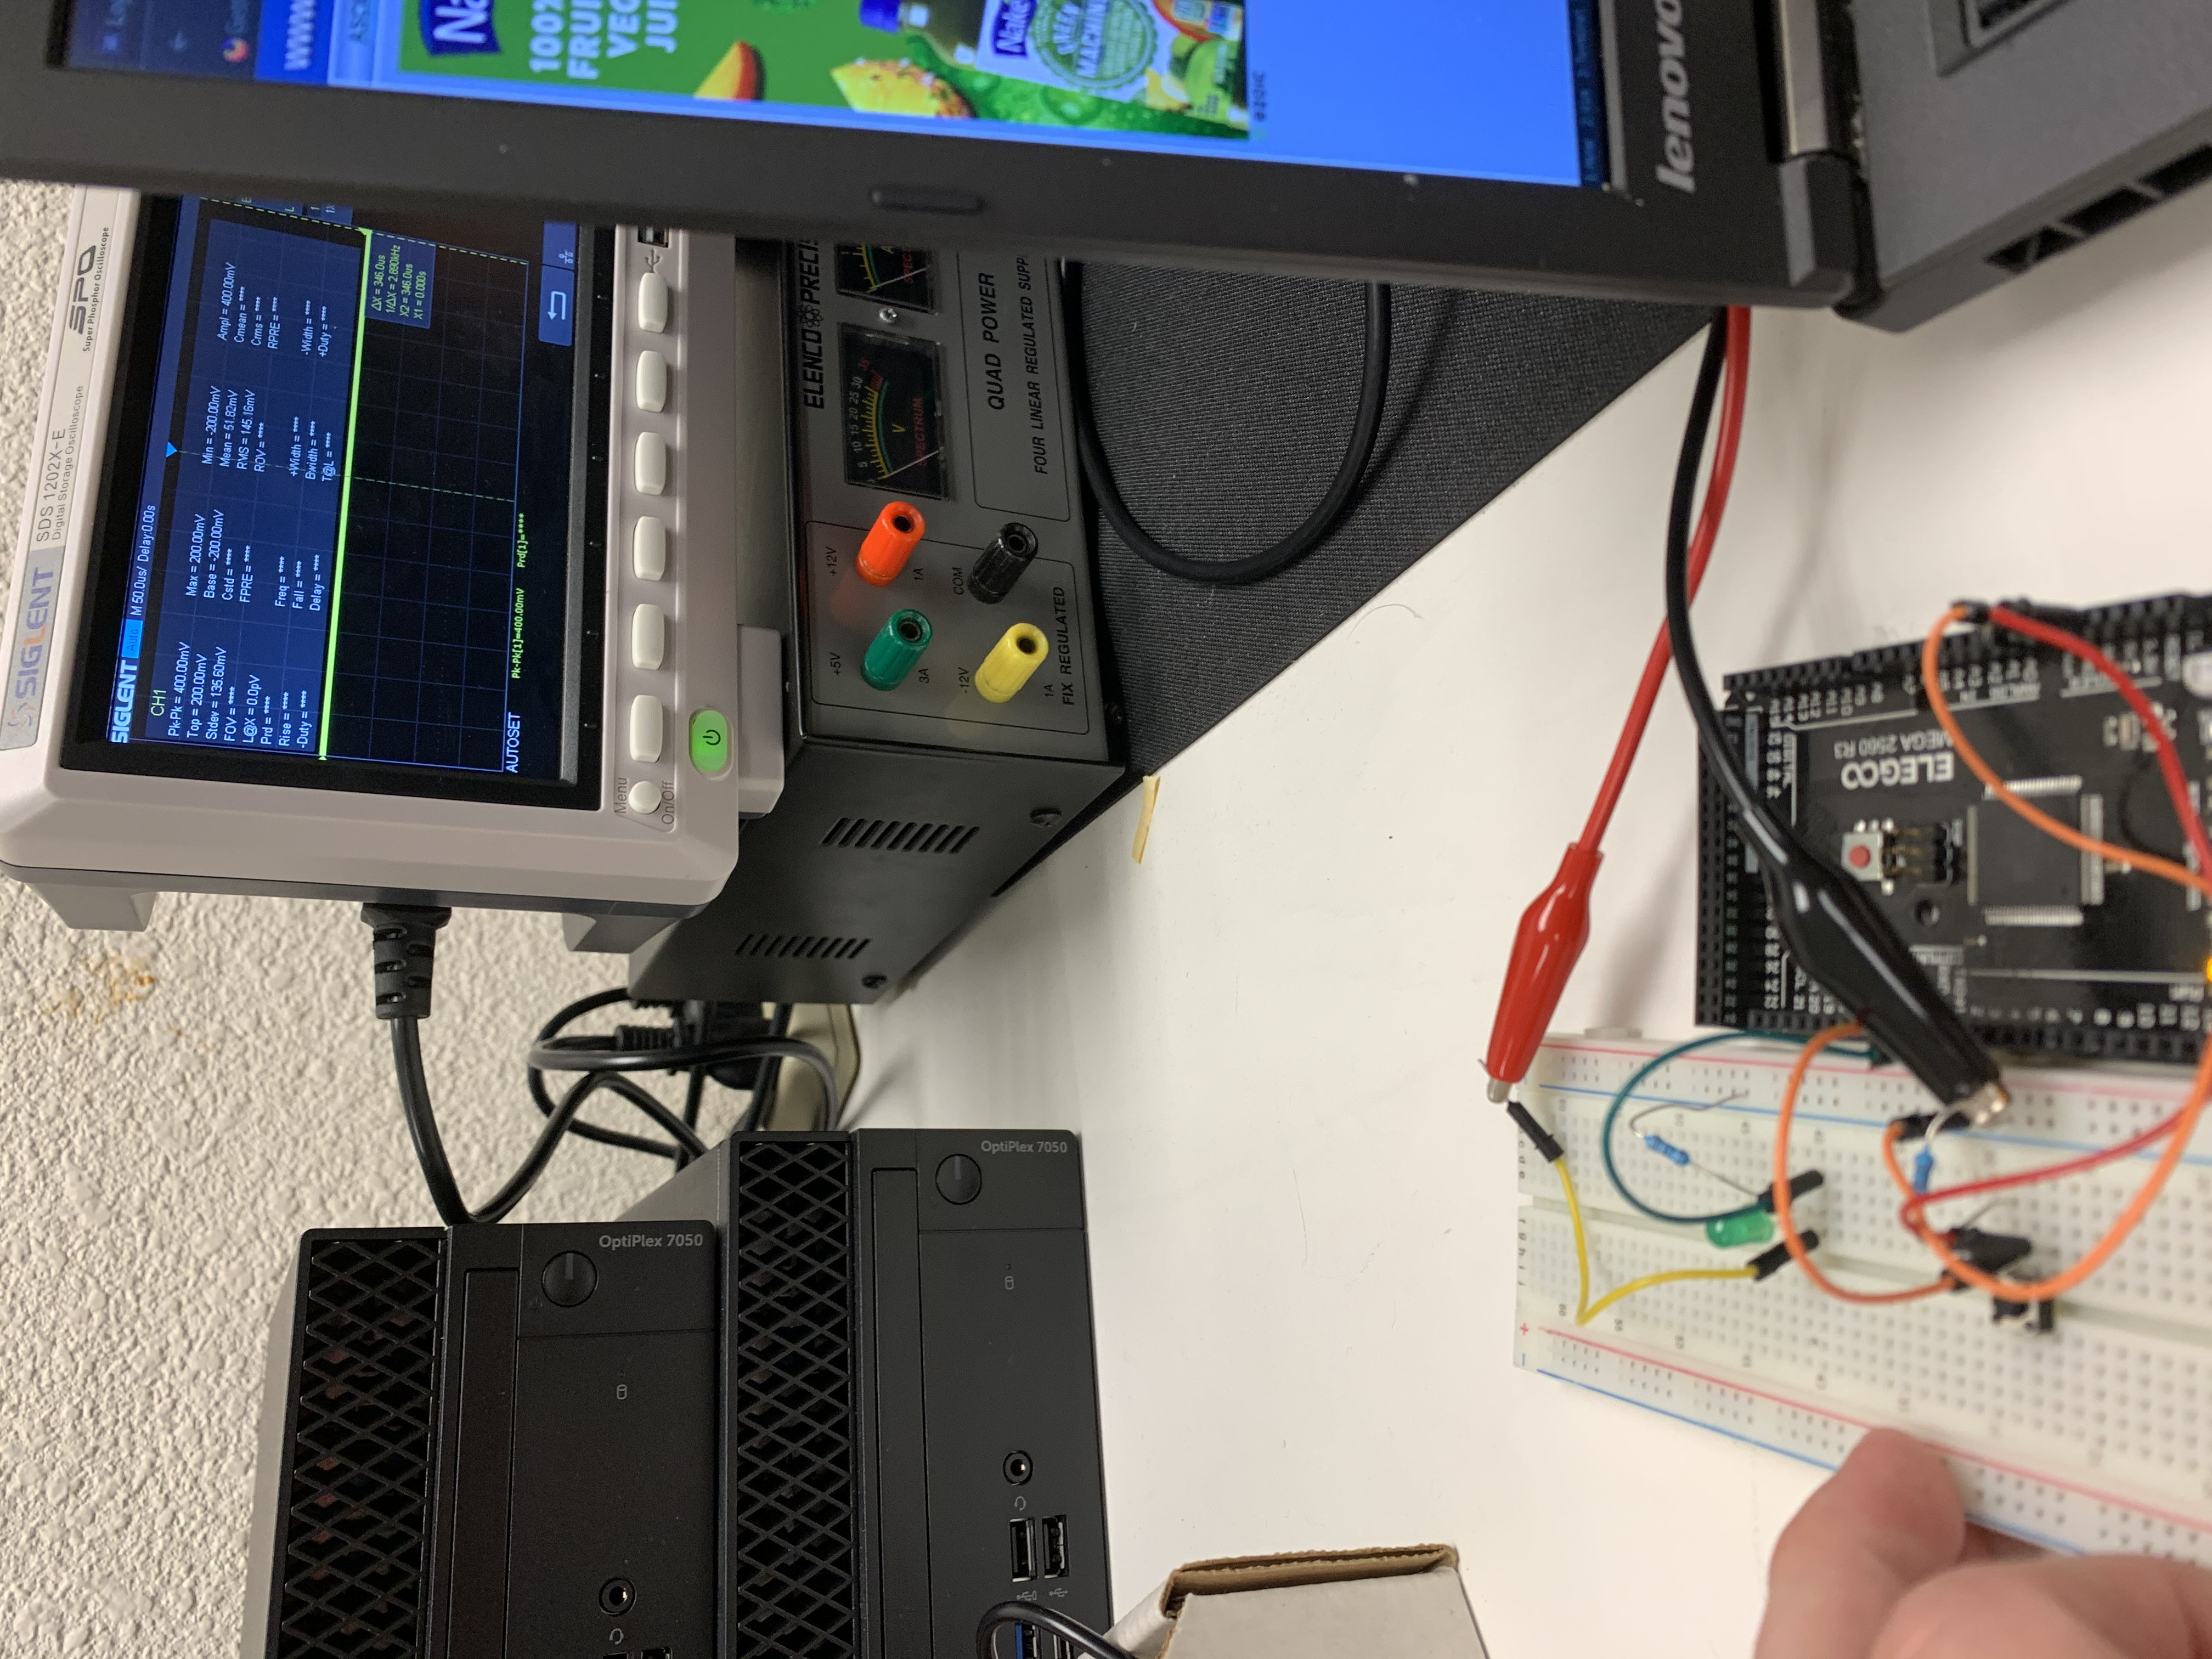
\includegraphics[scale=.06,angle=-90]{4.jpg}\\
	\item The Oscilloscope reads $\approx4.6V-5V$ when pressed.\\
	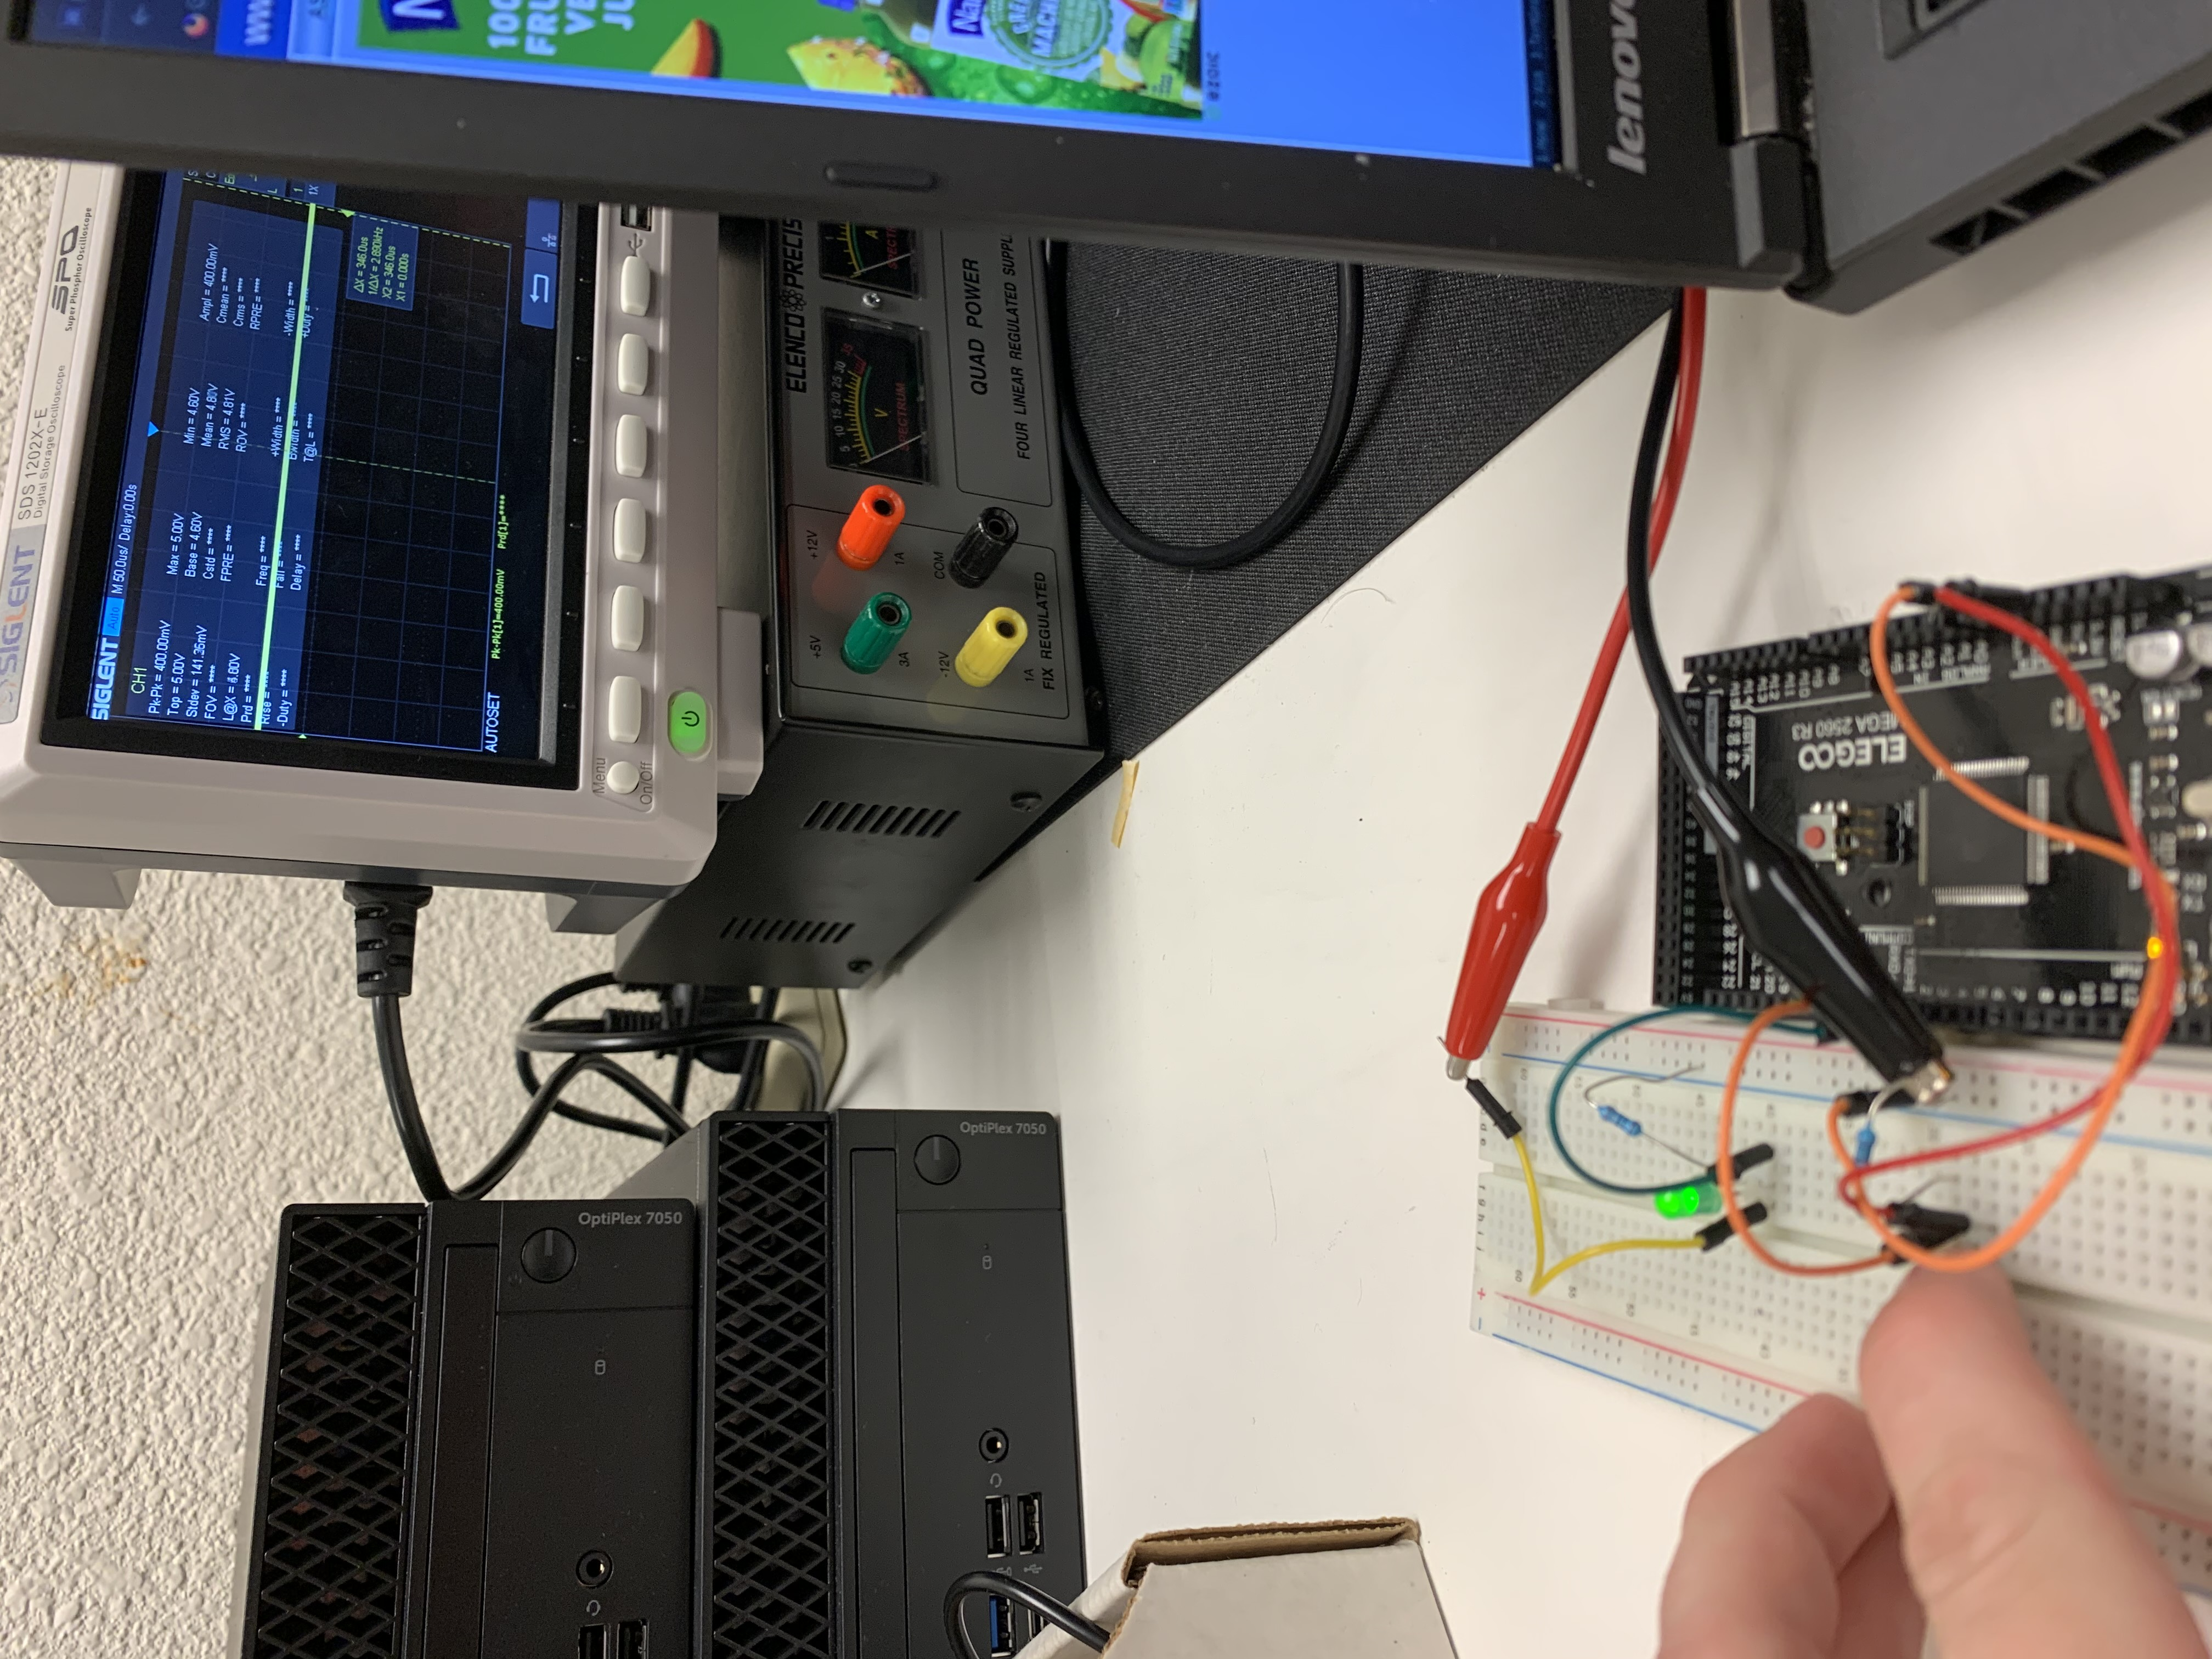
\includegraphics[scale=.06,angle=-90]{5.jpg}\\
	\item This is due to us writing to the DDR and PORT register telling the IC to allow power to travel through that pin.
\end{enumerate}

\end{document}
